\documentclass[twoside]{book}

% Packages required by doxygen
\usepackage{fixltx2e}
\usepackage{calc}
\usepackage{doxygen}
\usepackage[export]{adjustbox} % also loads graphicx
\usepackage{graphicx}
\usepackage[utf8]{inputenc}
\usepackage{makeidx}
\usepackage{multicol}
\usepackage{multirow}
\PassOptionsToPackage{warn}{textcomp}
\usepackage{textcomp}
\usepackage[nointegrals]{wasysym}
\usepackage[table]{xcolor}

% Font selection
\usepackage[T1]{fontenc}
\usepackage[scaled=.90]{helvet}
\usepackage{courier}
\usepackage{amssymb}
\usepackage{sectsty}
\renewcommand{\familydefault}{\sfdefault}
\allsectionsfont{%
  \fontseries{bc}\selectfont%
  \color{darkgray}%
}
\renewcommand{\DoxyLabelFont}{%
  \fontseries{bc}\selectfont%
  \color{darkgray}%
}
\newcommand{\+}{\discretionary{\mbox{\scriptsize$\hookleftarrow$}}{}{}}

% Page & text layout
\usepackage{geometry}
\geometry{%
  a4paper,%
  top=2.5cm,%
  bottom=2.5cm,%
  left=2.5cm,%
  right=2.5cm%
}
\tolerance=750
\hfuzz=15pt
\hbadness=750
\setlength{\emergencystretch}{15pt}
\setlength{\parindent}{0cm}
\setlength{\parskip}{3ex plus 2ex minus 2ex}
\makeatletter
\renewcommand{\paragraph}{%
  \@startsection{paragraph}{4}{0ex}{-1.0ex}{1.0ex}{%
    \normalfont\normalsize\bfseries\SS@parafont%
  }%
}
\renewcommand{\subparagraph}{%
  \@startsection{subparagraph}{5}{0ex}{-1.0ex}{1.0ex}{%
    \normalfont\normalsize\bfseries\SS@subparafont%
  }%
}
\makeatother

% Headers & footers
\usepackage{fancyhdr}
\pagestyle{fancyplain}
\fancyhead[LE]{\fancyplain{}{\bfseries\thepage}}
\fancyhead[CE]{\fancyplain{}{}}
\fancyhead[RE]{\fancyplain{}{\bfseries\leftmark}}
\fancyhead[LO]{\fancyplain{}{\bfseries\rightmark}}
\fancyhead[CO]{\fancyplain{}{}}
\fancyhead[RO]{\fancyplain{}{\bfseries\thepage}}
\fancyfoot[LE]{\fancyplain{}{}}
\fancyfoot[CE]{\fancyplain{}{}}
\fancyfoot[RE]{\fancyplain{}{\bfseries\scriptsize Generated by Doxygen }}
\fancyfoot[LO]{\fancyplain{}{\bfseries\scriptsize Generated by Doxygen }}
\fancyfoot[CO]{\fancyplain{}{}}
\fancyfoot[RO]{\fancyplain{}{}}
\renewcommand{\footrulewidth}{0.4pt}
\renewcommand{\chaptermark}[1]{%
  \markboth{#1}{}%
}
\renewcommand{\sectionmark}[1]{%
  \markright{\thesection\ #1}%
}

% Indices & bibliography
\usepackage{natbib}
\usepackage[titles]{tocloft}
\setcounter{tocdepth}{3}
\setcounter{secnumdepth}{5}
\makeindex

% Hyperlinks (required, but should be loaded last)
\usepackage{ifpdf}
\ifpdf
  \usepackage[pdftex,pagebackref=true]{hyperref}
\else
  \usepackage[ps2pdf,pagebackref=true]{hyperref}
\fi
\hypersetup{%
  colorlinks=true,%
  linkcolor=blue,%
  citecolor=blue,%
  unicode%
}

% Custom commands
\newcommand{\clearemptydoublepage}{%
  \newpage{\pagestyle{empty}\cleardoublepage}%
}

\usepackage{caption}
\captionsetup{labelsep=space,justification=centering,font={bf},singlelinecheck=off,skip=4pt,position=top}

%===== C O N T E N T S =====

\begin{document}

% Titlepage & ToC
\hypersetup{pageanchor=false,
             bookmarksnumbered=true,
             pdfencoding=unicode
            }
\pagenumbering{alph}
\begin{titlepage}
\vspace*{7cm}
\begin{center}%
{\Large Tokenika eosc \\[1ex]\large 0.\+5 }\\
\vspace*{1cm}
{\large Generated by Doxygen 1.8.13}\\
\end{center}
\end{titlepage}
\clearemptydoublepage
\pagenumbering{roman}
\tableofcontents
\clearemptydoublepage
\pagenumbering{arabic}
\hypersetup{pageanchor=true}

%--- Begin generated contents ---
\chapter{Module Index}
\section{Modules}
Here is a list of all modules\+:\begin{DoxyCompactList}
\item \contentsline{section}{Tokenika-\/\+E\+OS Command Line Client Reference}{\pageref{group__eosc}}{}
\end{DoxyCompactList}

\chapter{Hierarchical Index}
\section{Class Hierarchy}
This inheritance list is sorted roughly, but not completely, alphabetically\+:\begin{DoxyCompactList}
\item \contentsline{section}{tokenika\+:\+:eosc\+:\+:Command\+Options}{\pageref{classtokenika_1_1eosc_1_1_command_options}}{}
\begin{DoxyCompactList}
\item \contentsline{section}{tokenika\+:\+:eosc\+:\+:get\+\_\+block\+Options}{\pageref{classtokenika_1_1eosc_1_1get__block_options}}{}
\item \contentsline{section}{tokenika\+:\+:eosc\+:\+:get\+\_\+info\+Options}{\pageref{classtokenika_1_1eosc_1_1get__info_options}}{}
\end{DoxyCompactList}
\item \contentsline{section}{tokenika\+:\+:eosc\+:\+:Eosc\+Command}{\pageref{classtokenika_1_1eosc_1_1_eosc_command}}{}
\begin{DoxyCompactList}
\item \contentsline{section}{tokenika\+:\+:eosc\+:\+:get\+\_\+block}{\pageref{classtokenika_1_1eosc_1_1get__block}}{}
\item \contentsline{section}{tokenika\+:\+:eosc\+:\+:get\+\_\+info}{\pageref{classtokenika_1_1eosc_1_1get__info}}{}
\end{DoxyCompactList}
\item \contentsline{section}{tokenika\+:\+:eosc\+:\+:Init\+Get\+Json}{\pageref{structtokenika_1_1eosc_1_1_init_get_json}}{}
\end{DoxyCompactList}

\chapter{Data Structure Index}
\section{Data Structures}
Here are the data structures with brief descriptions\+:\begin{DoxyCompactList}
\item\contentsline{section}{\hyperlink{classtokenika_1_1eosc_1_1_command_options}{tokenika\+::eosc\+::\+Command\+Options} \\*Command-\/line wrapper for eosc commands }{\pageref{classtokenika_1_1eosc_1_1_command_options}}{}
\item\contentsline{section}{\hyperlink{classtokenika_1_1eosc_1_1_eosc_command}{tokenika\+::eosc\+::\+Eosc\+Command} \\*Basic connection to the blockchain }{\pageref{classtokenika_1_1eosc_1_1_eosc_command}}{}
\item\contentsline{section}{\hyperlink{classtokenika_1_1eosc_1_1_get_block}{tokenika\+::eosc\+::\+Get\+Block} \\*Retrieve a full block from a blockchain }{\pageref{classtokenika_1_1eosc_1_1_get_block}}{}
\item\contentsline{section}{\hyperlink{classtokenika_1_1eosc_1_1_get_block_options}{tokenika\+::eosc\+::\+Get\+Block\+Options} }{\pageref{classtokenika_1_1eosc_1_1_get_block_options}}{}
\item\contentsline{section}{\hyperlink{classtokenika_1_1eosc_1_1_get_info}{tokenika\+::eosc\+::\+Get\+Info} \\*Get current blockchain information }{\pageref{classtokenika_1_1eosc_1_1_get_info}}{}
\item\contentsline{section}{\hyperlink{classtokenika_1_1eosc_1_1_get_info_options}{tokenika\+::eosc\+::\+Get\+Info\+Options} }{\pageref{classtokenika_1_1eosc_1_1_get_info_options}}{}
\item\contentsline{section}{\hyperlink{structtokenika_1_1eosc_1_1_init_get_json}{tokenika\+::eosc\+::\+Init\+Get\+Json} }{\pageref{structtokenika_1_1eosc_1_1_init_get_json}}{}
\end{DoxyCompactList}

\chapter{File Index}
\section{File List}
Here is a list of all documented files with brief descriptions\+:\begin{DoxyCompactList}
\item\contentsline{section}{\hyperlink{eosc__command_8hpp}{eosc\+\_\+command.\+hpp} \\*Tool for sending transactions and querying state from E\+OS blockchain }{\pageref{eosc__command_8hpp}}{}
\item\contentsline{section}{\hyperlink{eosc__get__commands_8hpp}{eosc\+\_\+get\+\_\+commands.\+hpp} }{\pageref{eosc__get__commands_8hpp}}{}
\end{DoxyCompactList}

\chapter{Module Documentation}
\hypertarget{group__eosc}{}\section{Tokenika-\/\+E\+OS Command Line Client Reference}
\label{group__eosc}\index{Tokenika-\/\+E\+O\+S Command Line Client Reference@{Tokenika-\/\+E\+O\+S Command Line Client Reference}}


Tool for sending transactions and querying state from E\+OS blockchain.  


Tool for sending transactions and querying state from E\+OS blockchain. 

Base definitions.

Defines base classes of the project, and helper methods. 
\chapter{Data Structure Documentation}
\hypertarget{classtokenika_1_1eosc_1_1_command_options}{}\section{tokenika\+:\+:eosc\+:\+:Command\+Options Class Reference}
\label{classtokenika_1_1eosc_1_1_command_options}\index{tokenika\+::eosc\+::\+Command\+Options@{tokenika\+::eosc\+::\+Command\+Options}}


Command line options base.  




{\ttfamily \#include $<$eosc\+\_\+command.\+hpp$>$}



Inheritance diagram for tokenika\+:\+:eosc\+:\+:Command\+Options\+:\nopagebreak
\begin{figure}[H]
\begin{center}
\leavevmode
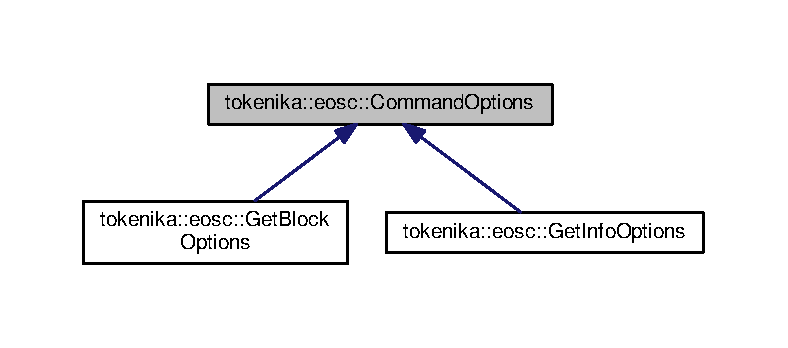
\includegraphics[width=350pt]{classtokenika_1_1eosc_1_1_command_options__inherit__graph}
\end{center}
\end{figure}
\subsection*{Public Member Functions}
\begin{DoxyCompactItemize}
\item 
\mbox{\Hypertarget{classtokenika_1_1eosc_1_1_command_options_a263a61f90aa324090e2d9d592b2d4ad6}\label{classtokenika_1_1eosc_1_1_command_options_a263a61f90aa324090e2d9d592b2d4ad6}} 
{\bfseries Command\+Options} (int argc, const char $\ast$$\ast$argv)
\item 
\mbox{\Hypertarget{classtokenika_1_1eosc_1_1_command_options_a4fa1c9defc45b139e415c79c43b15e5d}\label{classtokenika_1_1eosc_1_1_command_options_a4fa1c9defc45b139e415c79c43b15e5d}} 
void {\bfseries go} ()
\end{DoxyCompactItemize}
\subsection*{Protected Member Functions}
\begin{DoxyCompactItemize}
\item 
\mbox{\Hypertarget{classtokenika_1_1eosc_1_1_command_options_a28fb680d7477e19e523367d2585655fb}\label{classtokenika_1_1eosc_1_1_command_options_a28fb680d7477e19e523367d2585655fb}} 
virtual const char $\ast$ {\bfseries get\+\_\+usage} ()
\item 
\mbox{\Hypertarget{classtokenika_1_1eosc_1_1_command_options_aa55960f380250eb7065cb6489b67196f}\label{classtokenika_1_1eosc_1_1_command_options_aa55960f380250eb7065cb6489b67196f}} 
virtual boost\+::program\+\_\+options\+::options\+\_\+description {\bfseries options} ()
\item 
\mbox{\Hypertarget{classtokenika_1_1eosc_1_1_command_options_a817eaab59b5815964bc496da2c1fa607}\label{classtokenika_1_1eosc_1_1_command_options_a817eaab59b5815964bc496da2c1fa607}} 
virtual void {\bfseries set\+\_\+pos\+\_\+desc} (boost\+::program\+\_\+options\+::positional\+\_\+options\+\_\+description \&pos\+\_\+descr)
\item 
\mbox{\Hypertarget{classtokenika_1_1eosc_1_1_command_options_a117ff5d9632d4d9f773f49a7e6936a67}\label{classtokenika_1_1eosc_1_1_command_options_a117ff5d9632d4d9f773f49a7e6936a67}} 
virtual bool {\bfseries set\+\_\+json} (boost\+::program\+\_\+options\+::variables\+\_\+map \&vm)
\item 
\mbox{\Hypertarget{classtokenika_1_1eosc_1_1_command_options_abc8896966d7f5772624aefade1e41013}\label{classtokenika_1_1eosc_1_1_command_options_abc8896966d7f5772624aefade1e41013}} 
virtual \hyperlink{classtokenika_1_1eosc_1_1_eosc_command}{Eosc\+Command} {\bfseries get\+\_\+command} (bool is\+Raw)
\item 
\mbox{\Hypertarget{classtokenika_1_1eosc_1_1_command_options_a39f81ab9ca094499d7b2f498af282b27}\label{classtokenika_1_1eosc_1_1_command_options_a39f81ab9ca094499d7b2f498af282b27}} 
virtual void {\bfseries get\+\_\+example} ()
\item 
\mbox{\Hypertarget{classtokenika_1_1eosc_1_1_command_options_a37b5801fa36d27bc606128162fccee00}\label{classtokenika_1_1eosc_1_1_command_options_a37b5801fa36d27bc606128162fccee00}} 
virtual void {\bfseries get\+\_\+output} (\hyperlink{classtokenika_1_1eosc_1_1_eosc_command}{Eosc\+Command} command)
\item 
\mbox{\Hypertarget{classtokenika_1_1eosc_1_1_command_options_aaa229149507991d88d71267d2552d20e}\label{classtokenika_1_1eosc_1_1_command_options_aaa229149507991d88d71267d2552d20e}} 
void {\bfseries common\+\_\+options} (boost\+::program\+\_\+options\+::options\+\_\+description \&common)
\end{DoxyCompactItemize}
\subsection*{Protected Attributes}
\begin{DoxyCompactItemize}
\item 
\mbox{\Hypertarget{classtokenika_1_1eosc_1_1_command_options_a626e842c89d8332090886bc53fbad616}\label{classtokenika_1_1eosc_1_1_command_options_a626e842c89d8332090886bc53fbad616}} 
boost\+::property\+\_\+tree\+::ptree {\bfseries post\+Json}
\end{DoxyCompactItemize}


\subsection{Detailed Description}
Command line options base. 

The documentation for this class was generated from the following files\+:\begin{DoxyCompactItemize}
\item 
\hyperlink{eosc__command_8hpp}{eosc\+\_\+command.\+hpp}\item 
eosc\+\_\+command.\+cpp\end{DoxyCompactItemize}

\hypertarget{classtokenika_1_1eosc_1_1_eosc_command}{}\section{tokenika\+:\+:eosc\+:\+:Eosc\+Command Class Reference}
\label{classtokenika_1_1eosc_1_1_eosc_command}\index{tokenika\+::eosc\+::\+Eosc\+Command@{tokenika\+::eosc\+::\+Eosc\+Command}}


Inheritance diagram for tokenika\+:\+:eosc\+:\+:Eosc\+Command\+:\nopagebreak
\begin{figure}[H]
\begin{center}
\leavevmode
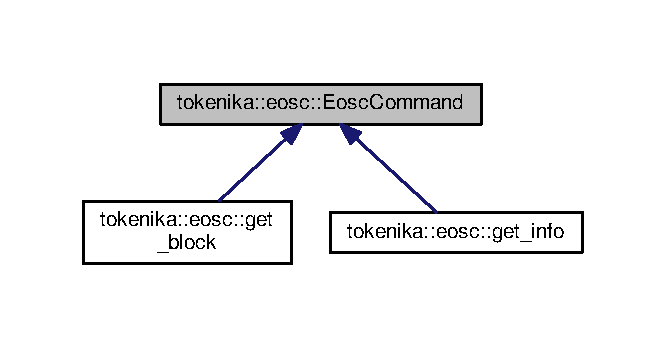
\includegraphics[width=344pt]{classtokenika_1_1eosc_1_1_eosc_command__inherit__graph}
\end{center}
\end{figure}
\subsection*{Public Member Functions}
\begin{DoxyCompactItemize}
\item 
\mbox{\Hypertarget{classtokenika_1_1eosc_1_1_eosc_command_ab736f0dcd8ca14eb0daf9b2244218397}\label{classtokenika_1_1eosc_1_1_eosc_command_ab736f0dcd8ca14eb0daf9b2244218397}} 
{\bfseries Eosc\+Command} (std\+::string path, boost\+::property\+\_\+tree\+::ptree post\+Json, bool is\+Raw=false)
\item 
\mbox{\Hypertarget{classtokenika_1_1eosc_1_1_eosc_command_ac9db6f0741086143353cdecb49e496dd}\label{classtokenika_1_1eosc_1_1_eosc_command_ac9db6f0741086143353cdecb49e496dd}} 
{\bfseries Eosc\+Command} (std\+::string path, std\+::string json, bool is\+Raw=false)
\item 
\mbox{\Hypertarget{classtokenika_1_1eosc_1_1_eosc_command_aa26a8e34b790074bb0a87b6fe82c29cb}\label{classtokenika_1_1eosc_1_1_eosc_command_aa26a8e34b790074bb0a87b6fe82c29cb}} 
void {\bfseries call\+\_\+eosd} ()
\item 
\mbox{\Hypertarget{classtokenika_1_1eosc_1_1_eosc_command_a63f3adace3f84b59f64c5a54ca0c18dc}\label{classtokenika_1_1eosc_1_1_eosc_command_a63f3adace3f84b59f64c5a54ca0c18dc}} 
bool {\bfseries is\+Error} () const
\item 
\mbox{\Hypertarget{classtokenika_1_1eosc_1_1_eosc_command_a2b451aefc95258d481cff16747fa1888}\label{classtokenika_1_1eosc_1_1_eosc_command_a2b451aefc95258d481cff16747fa1888}} 
boost\+::property\+\_\+tree\+::ptree {\bfseries get\+Rcv\+Json} () const
\item 
\mbox{\Hypertarget{classtokenika_1_1eosc_1_1_eosc_command_a1cb0362dceb5999e7e06078223b20d91}\label{classtokenika_1_1eosc_1_1_eosc_command_a1cb0362dceb5999e7e06078223b20d91}} 
std\+::string {\bfseries to\+String\+Post} () const
\item 
\mbox{\Hypertarget{classtokenika_1_1eosc_1_1_eosc_command_ad01ef46444d9d8bc708b5d18605c3903}\label{classtokenika_1_1eosc_1_1_eosc_command_ad01ef46444d9d8bc708b5d18605c3903}} 
std\+::string {\bfseries to\+String\+Rcv} () const
\item 
{\footnotesize template$<$typename Type $>$ }\\Type \hyperlink{classtokenika_1_1eosc_1_1_eosc_command_aa1da6eb23f52159afa4a15e767cd7d6f}{get} (const boost\+::property\+\_\+tree\+::ptree\+::path\+\_\+type \&path) const
\begin{DoxyCompactList}\small\item\em Returns a value of a path of the received json. \end{DoxyCompactList}\end{DoxyCompactItemize}
\subsection*{Protected Attributes}
\begin{DoxyCompactItemize}
\item 
\mbox{\Hypertarget{classtokenika_1_1eosc_1_1_eosc_command_a1642782c91f4877a8fba395324fb7337}\label{classtokenika_1_1eosc_1_1_eosc_command_a1642782c91f4877a8fba395324fb7337}} 
boost\+::property\+\_\+tree\+::ptree {\bfseries post\+Json}
\end{DoxyCompactItemize}


\subsection{Member Function Documentation}
\mbox{\Hypertarget{classtokenika_1_1eosc_1_1_eosc_command_aa1da6eb23f52159afa4a15e767cd7d6f}\label{classtokenika_1_1eosc_1_1_eosc_command_aa1da6eb23f52159afa4a15e767cd7d6f}} 
\index{tokenika\+::eosc\+::\+Eosc\+Command@{tokenika\+::eosc\+::\+Eosc\+Command}!get@{get}}
\index{get@{get}!tokenika\+::eosc\+::\+Eosc\+Command@{tokenika\+::eosc\+::\+Eosc\+Command}}
\subsubsection{\texorpdfstring{get()}{get()}}
{\footnotesize\ttfamily template$<$typename Type $>$ \\
Type tokenika\+::eosc\+::\+Eosc\+Command\+::get (\begin{DoxyParamCaption}\item[{const boost\+::property\+\_\+tree\+::ptree\+::path\+\_\+type \&}]{path }\end{DoxyParamCaption}) const\hspace{0.3cm}{\ttfamily [inline]}}



Returns a value of a path of the received json. 


\begin{DoxyTemplParams}{Template Parameters}
{\em Type} & \\
\hline
\end{DoxyTemplParams}

\begin{DoxyParams}{Parameters}
{\em path} & \\
\hline
\end{DoxyParams}
\begin{DoxyReturn}{Returns}
Type get 
\end{DoxyReturn}


The documentation for this class was generated from the following files\+:\begin{DoxyCompactItemize}
\item 
\hyperlink{eosc__command_8hpp}{eosc\+\_\+command.\+hpp}\item 
eosc\+\_\+command.\+cpp\end{DoxyCompactItemize}

\hypertarget{classtokenika_1_1eosc_1_1_get_block}{}\section{tokenika\+:\+:eosc\+:\+:Get\+Block Class Reference}
\label{classtokenika_1_1eosc_1_1_get_block}\index{tokenika\+::eosc\+::\+Get\+Block@{tokenika\+::eosc\+::\+Get\+Block}}


Retrieve a full block from a blockchain.  




{\ttfamily \#include $<$eosc\+\_\+get\+\_\+commands.\+hpp$>$}



Inheritance diagram for tokenika\+:\+:eosc\+:\+:Get\+Block\+:
\nopagebreak
\begin{figure}[H]
\begin{center}
\leavevmode
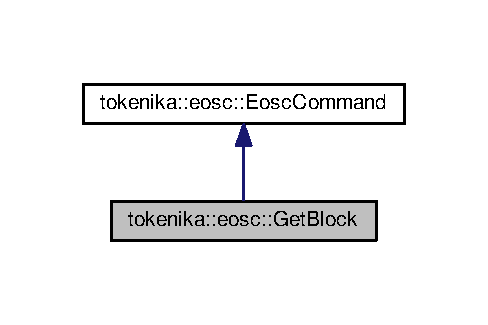
\includegraphics[width=234pt]{classtokenika_1_1eosc_1_1_get_block__inherit__graph}
\end{center}
\end{figure}


Collaboration diagram for tokenika\+:\+:eosc\+:\+:Get\+Block\+:
\nopagebreak
\begin{figure}[H]
\begin{center}
\leavevmode
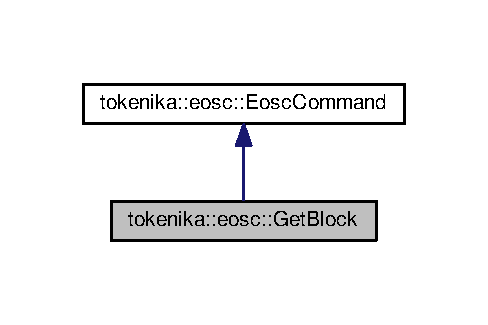
\includegraphics[width=234pt]{classtokenika_1_1eosc_1_1_get_block__coll__graph}
\end{center}
\end{figure}
\subsection*{Public Member Functions}
\begin{DoxyCompactItemize}
\item 
\mbox{\Hypertarget{classtokenika_1_1eosc_1_1_get_block_a67c1536e676f26b9e9dac915092f9627}\label{classtokenika_1_1eosc_1_1_get_block_a67c1536e676f26b9e9dac915092f9627}} 
{\bfseries Get\+Block} (boost\+::property\+\_\+tree\+::ptree post\+Json, bool raw=false)
\end{DoxyCompactItemize}
\subsection*{Additional Inherited Members}


\subsection{Detailed Description}
Retrieve a full block from a blockchain. 

Given a {\ttfamily boost\+::property\+\_\+tree\+::ptree json}, conforms (\href{#https://github.com/EOSIO/eosjs-json/blob/master/api/v1/chain.json}{\tt after eosjs-\/json}) this pattern\+: \begin{DoxyVerb}* {"block_num_or_id":"uint32 | string"}.
* \end{DoxyVerb}


the constructor posts it to an E\+OS block socket, specified in the {\ttfamily eosc\+\_\+config.\+json} file. The responce of the blockchain is, again, a {\ttfamily boost\+::property\+\_\+tree\+::ptree json}. On error, the reaponce json is {\ttfamily \{\char`\"{}error\char`\"{}\+:\char`\"{}error message\char`\"{}\}}, otherwise it conforms (\href{#https://github.com/EOSIO/eosjs-json/blob/master/api/v1/chain.json}{\tt after eosjs-\/json}) this pattern\+: \begin{DoxyVerb}* {
* "previous":"uint32",
* "timestamp":"2017-07-18T20:16:36",
* "transaction_merkle_root":"uint32",
* "producer":"uint16",
* "producer_changes":"map<account_name, account_name>[]",
* "producer_signature":"signature",
* "cycles":"thread[]",
* "id":"fixed_bytes33",
* "block_num":"uint32",
* "refBlockPrefix":"uint32"
* }
* \end{DoxyVerb}


It is available with the \hyperlink{classtokenika_1_1eosc_1_1_eosc_command_a2b451aefc95258d481cff16747fa1888}{tokenika\+::eosc\+::\+Eosc\+Command\+::get\+Rcv\+Json()} method.

Note that time is a string. For processing, it has to be expressed as a structure and afterwords back to a string. Helper functions, namely \+::str\+To\+Time(const std\+::string)

Example\+:

\begin{DoxyVerb}* #include <stdio.h>
* #include <stdlib.h>
* #include <iostream>
* #include <string>
* 
* #include <boost/property_tree/ptree.hpp>
* #include "boost/date_time/posix_time/posix_time.hpp"
* 
* #include "EoscCommands/eosc_get_commands.hpp"  
* 
* int main(int argc, char *argv[])
* {
* boost::property_tree::ptree postJson;
* postJson.put("block_num_or_id", 25);
* tokenika::eosc::GetBlock getBlock(getInfoPostJson);
* if(!getBlock.isError())
* {
*    std::cout << getBlock.get<int>("last_irreversible_block_num")) << std::endl;
*    boost::posix_time::ptime time = GetInfo.get<boost::posix_time::ptime>("timestamp");
*    std::cout << time << std::endl;
*    boost::posix_time::ptime t1 = time + boost::posix_time::seconds(900);
*    cout << (boost::posix_time::to_iso_extended_string)(t1) << endl;
* } else
* {
*    std::cerr << getBlock.get<string>("error")) << std::endl;
* }
* 
* return 0;
* }
* \end{DoxyVerb}
 

The documentation for this class was generated from the following file\+:\begin{DoxyCompactItemize}
\item 
eosc\+\_\+get\+\_\+commands.\+hpp\end{DoxyCompactItemize}

\hypertarget{classtokenika_1_1eosc_1_1_get_block_options}{}\section{tokenika\+:\+:eosc\+:\+:Get\+Block\+Options Class Reference}
\label{classtokenika_1_1eosc_1_1_get_block_options}\index{tokenika\+::eosc\+::\+Get\+Block\+Options@{tokenika\+::eosc\+::\+Get\+Block\+Options}}


Inheritance diagram for tokenika\+:\+:eosc\+:\+:Get\+Block\+Options\+:\nopagebreak
\begin{figure}[H]
\begin{center}
\leavevmode
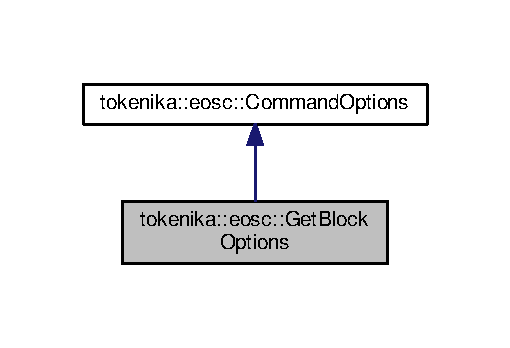
\includegraphics[width=245pt]{classtokenika_1_1eosc_1_1_get_block_options__inherit__graph}
\end{center}
\end{figure}


Collaboration diagram for tokenika\+:\+:eosc\+:\+:Get\+Block\+Options\+:\nopagebreak
\begin{figure}[H]
\begin{center}
\leavevmode
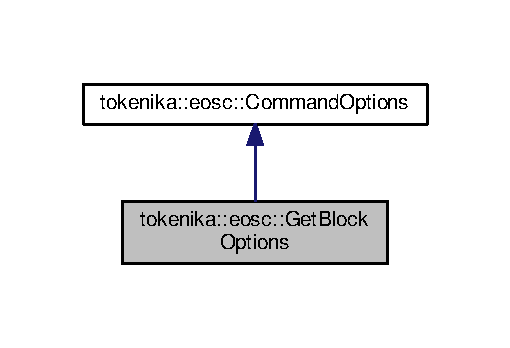
\includegraphics[width=245pt]{classtokenika_1_1eosc_1_1_get_block_options__coll__graph}
\end{center}
\end{figure}
\subsection*{Public Member Functions}
\begin{DoxyCompactItemize}
\item 
\mbox{\Hypertarget{classtokenika_1_1eosc_1_1_get_block_options_ab031795a5bd5cf681307cc9ea07659a3}\label{classtokenika_1_1eosc_1_1_get_block_options_ab031795a5bd5cf681307cc9ea07659a3}} 
{\bfseries Get\+Block\+Options} (int argc, const char $\ast$$\ast$argv)
\end{DoxyCompactItemize}
\subsection*{Protected Member Functions}
\begin{DoxyCompactItemize}
\item 
\mbox{\Hypertarget{classtokenika_1_1eosc_1_1_get_block_options_aed0e156ee7251256d9b52a07f590c0d3}\label{classtokenika_1_1eosc_1_1_get_block_options_aed0e156ee7251256d9b52a07f590c0d3}} 
const char $\ast$ {\bfseries get\+\_\+usage} ()
\item 
\mbox{\Hypertarget{classtokenika_1_1eosc_1_1_get_block_options_a6e8c1a240e5a529c093e0053f12e9ee5}\label{classtokenika_1_1eosc_1_1_get_block_options_a6e8c1a240e5a529c093e0053f12e9ee5}} 
virtual boost\+::program\+\_\+options\+::options\+\_\+description {\bfseries options} ()
\item 
\mbox{\Hypertarget{classtokenika_1_1eosc_1_1_get_block_options_a8455d8ad48f073736576dc6b74de664d}\label{classtokenika_1_1eosc_1_1_get_block_options_a8455d8ad48f073736576dc6b74de664d}} 
virtual void {\bfseries set\+\_\+pos\+\_\+desc} (boost\+::program\+\_\+options\+::positional\+\_\+options\+\_\+description \&pos\+\_\+desc)
\item 
\mbox{\Hypertarget{classtokenika_1_1eosc_1_1_get_block_options_a0e2e25029e13410b7ca60369818d0789}\label{classtokenika_1_1eosc_1_1_get_block_options_a0e2e25029e13410b7ca60369818d0789}} 
virtual bool {\bfseries set\+\_\+json} (boost\+::program\+\_\+options\+::variables\+\_\+map \&vm)
\item 
\mbox{\Hypertarget{classtokenika_1_1eosc_1_1_get_block_options_ac391b4b079f7e461e9413c68c3ab3ae5}\label{classtokenika_1_1eosc_1_1_get_block_options_ac391b4b079f7e461e9413c68c3ab3ae5}} 
virtual \hyperlink{classtokenika_1_1eosc_1_1_eosc_command}{Eosc\+Command} {\bfseries get\+\_\+command} (bool is\+\_\+raw)
\item 
\mbox{\Hypertarget{classtokenika_1_1eosc_1_1_get_block_options_ac7eb6dfe97da31f169f21862f6fe84ea}\label{classtokenika_1_1eosc_1_1_get_block_options_ac7eb6dfe97da31f169f21862f6fe84ea}} 
virtual void {\bfseries get\+\_\+output} (\hyperlink{classtokenika_1_1eosc_1_1_eosc_command}{Eosc\+Command} command)
\item 
\mbox{\Hypertarget{classtokenika_1_1eosc_1_1_get_block_options_a609df79f796fc08b357d81632869fc6a}\label{classtokenika_1_1eosc_1_1_get_block_options_a609df79f796fc08b357d81632869fc6a}} 
virtual void {\bfseries get\+\_\+example} ()
\end{DoxyCompactItemize}
\subsection*{Protected Attributes}
\begin{DoxyCompactItemize}
\item 
\mbox{\Hypertarget{classtokenika_1_1eosc_1_1_get_block_options_af6c20effd6a52b8d26a8377450585142}\label{classtokenika_1_1eosc_1_1_get_block_options_af6c20effd6a52b8d26a8377450585142}} 
int {\bfseries n}
\item 
\mbox{\Hypertarget{classtokenika_1_1eosc_1_1_get_block_options_a0eda5e812218067adfc5bbab2d6b4048}\label{classtokenika_1_1eosc_1_1_get_block_options_a0eda5e812218067adfc5bbab2d6b4048}} 
std\+::string {\bfseries id}
\end{DoxyCompactItemize}


The documentation for this class was generated from the following file\+:\begin{DoxyCompactItemize}
\item 
eosc\+\_\+get\+\_\+commands.\+hpp\end{DoxyCompactItemize}

\hypertarget{classtokenika_1_1eosc_1_1_get_info}{}\section{tokenika\+:\+:eosc\+:\+:Get\+Info Class Reference}
\label{classtokenika_1_1eosc_1_1_get_info}\index{tokenika\+::eosc\+::\+Get\+Info@{tokenika\+::eosc\+::\+Get\+Info}}


Get current blockchain information.  




{\ttfamily \#include $<$eosc\+\_\+get\+\_\+commands.\+hpp$>$}



Inheritance diagram for tokenika\+:\+:eosc\+:\+:Get\+Info\+:\nopagebreak
\begin{figure}[H]
\begin{center}
\leavevmode
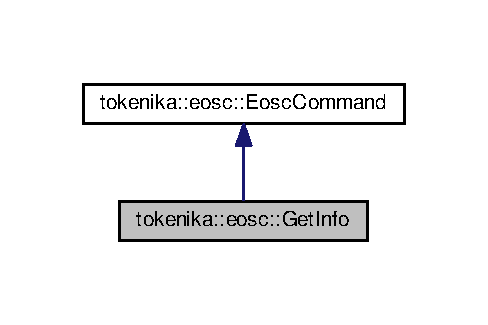
\includegraphics[width=234pt]{classtokenika_1_1eosc_1_1_get_info__inherit__graph}
\end{center}
\end{figure}


Collaboration diagram for tokenika\+:\+:eosc\+:\+:Get\+Info\+:\nopagebreak
\begin{figure}[H]
\begin{center}
\leavevmode
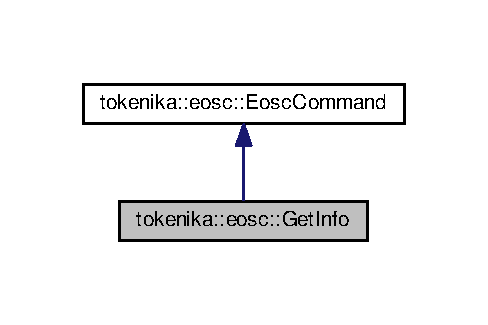
\includegraphics[width=234pt]{classtokenika_1_1eosc_1_1_get_info__coll__graph}
\end{center}
\end{figure}
\subsection*{Public Member Functions}
\begin{DoxyCompactItemize}
\item 
\mbox{\Hypertarget{classtokenika_1_1eosc_1_1_get_info_a3b219ff2f0036acbecf97922e28c3793}\label{classtokenika_1_1eosc_1_1_get_info_a3b219ff2f0036acbecf97922e28c3793}} 
{\bfseries Get\+Info} (boost\+::property\+\_\+tree\+::ptree post\+Json, bool raw=false)
\end{DoxyCompactItemize}
\subsection*{Additional Inherited Members}


\subsection{Detailed Description}
Get current blockchain information. 

Example\+:

\begin{DoxyVerb}* #include <stdio.h>
* #include <stdlib.h>
* #include <iostream>
* #include <string>
* #include <boost/property_tree/ptree.hpp>
* #include "EoscCommands/eosc_get_commands.hpp"
* 
* int main(int argc, char *argv[])
* {
* boost::property_tree::ptree postJson;
* tokenika::eosc::GetInfo GetInfo(getInfoPostJson);
* std::cout << GetInfo.get<int>("last_irreversible_block_num")) << std::endl;
* boost::property_tree::ptree rcv_json = GetInfo.getRcvJson();
* std::cout << GetBlock.toStringRcv() << std::endl; // Print the response json.
* 
* return 0;
* }
* \end{DoxyVerb}
 

The documentation for this class was generated from the following file\+:\begin{DoxyCompactItemize}
\item 
\hyperlink{eosc__get__commands_8hpp}{eosc\+\_\+get\+\_\+commands.\+hpp}\end{DoxyCompactItemize}

\hypertarget{classtokenika_1_1eosc_1_1_get_info_options}{}\section{tokenika\+:\+:eosc\+:\+:Get\+Info\+Options Class Reference}
\label{classtokenika_1_1eosc_1_1_get_info_options}\index{tokenika\+::eosc\+::\+Get\+Info\+Options@{tokenika\+::eosc\+::\+Get\+Info\+Options}}


Inheritance diagram for tokenika\+:\+:eosc\+:\+:Get\+Info\+Options\+:\nopagebreak
\begin{figure}[H]
\begin{center}
\leavevmode
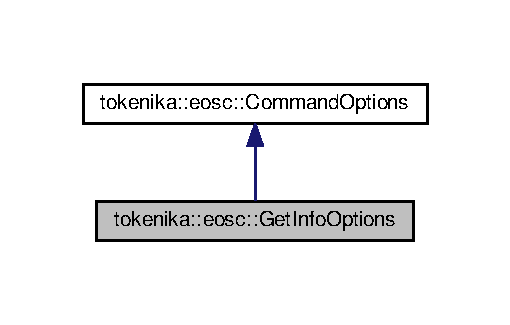
\includegraphics[width=245pt]{classtokenika_1_1eosc_1_1_get_info_options__inherit__graph}
\end{center}
\end{figure}


Collaboration diagram for tokenika\+:\+:eosc\+:\+:Get\+Info\+Options\+:\nopagebreak
\begin{figure}[H]
\begin{center}
\leavevmode
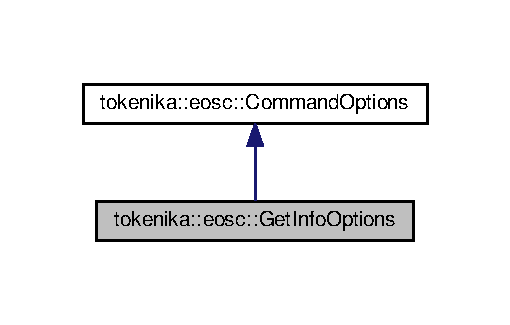
\includegraphics[width=245pt]{classtokenika_1_1eosc_1_1_get_info_options__coll__graph}
\end{center}
\end{figure}
\subsection*{Public Member Functions}
\begin{DoxyCompactItemize}
\item 
\mbox{\Hypertarget{classtokenika_1_1eosc_1_1_get_info_options_a9d3325947476e5eb6f3a44ebd28c02d8}\label{classtokenika_1_1eosc_1_1_get_info_options_a9d3325947476e5eb6f3a44ebd28c02d8}} 
{\bfseries Get\+Info\+Options} (int argc, const char $\ast$$\ast$argv)
\end{DoxyCompactItemize}
\subsection*{Protected Member Functions}
\begin{DoxyCompactItemize}
\item 
\mbox{\Hypertarget{classtokenika_1_1eosc_1_1_get_info_options_a05dff84e787d0de8a868675a1c4bdaf7}\label{classtokenika_1_1eosc_1_1_get_info_options_a05dff84e787d0de8a868675a1c4bdaf7}} 
const char $\ast$ {\bfseries get\+\_\+usage} ()
\item 
\mbox{\Hypertarget{classtokenika_1_1eosc_1_1_get_info_options_a1e9442163033df583c0e88a8bb7e2449}\label{classtokenika_1_1eosc_1_1_get_info_options_a1e9442163033df583c0e88a8bb7e2449}} 
virtual bool {\bfseries set\+\_\+json} (boost\+::program\+\_\+options\+::variables\+\_\+map \&vm)
\item 
\mbox{\Hypertarget{classtokenika_1_1eosc_1_1_get_info_options_a86c644c64a49731a043e28cef9d1c4d3}\label{classtokenika_1_1eosc_1_1_get_info_options_a86c644c64a49731a043e28cef9d1c4d3}} 
virtual \hyperlink{classtokenika_1_1eosc_1_1_eosc_command}{Eosc\+Command} {\bfseries get\+\_\+command} (bool is\+\_\+raw)
\item 
\mbox{\Hypertarget{classtokenika_1_1eosc_1_1_get_info_options_ac5ed969c967312b99027f5ef8b8ae447}\label{classtokenika_1_1eosc_1_1_get_info_options_ac5ed969c967312b99027f5ef8b8ae447}} 
virtual void {\bfseries get\+\_\+output} (\hyperlink{classtokenika_1_1eosc_1_1_eosc_command}{tokenika\+::eosc\+::\+Eosc\+Command} command)
\item 
\mbox{\Hypertarget{classtokenika_1_1eosc_1_1_get_info_options_af7a45f9570c6dd7903e1ab525cc36487}\label{classtokenika_1_1eosc_1_1_get_info_options_af7a45f9570c6dd7903e1ab525cc36487}} 
virtual void {\bfseries get\+\_\+example} ()
\end{DoxyCompactItemize}
\subsection*{Additional Inherited Members}


The documentation for this class was generated from the following file\+:\begin{DoxyCompactItemize}
\item 
eosc\+\_\+get\+\_\+commands.\+hpp\end{DoxyCompactItemize}

\hypertarget{structtokenika_1_1eosc_1_1init__get1}{}\section{tokenika\+:\+:eosc\+:\+:init\+\_\+get1 Struct Reference}
\label{structtokenika_1_1eosc_1_1init__get1}\index{tokenika\+::eosc\+::init\+\_\+get1@{tokenika\+::eosc\+::init\+\_\+get1}}
\subsection*{Data Fields}
\begin{DoxyCompactItemize}
\item 
\mbox{\Hypertarget{structtokenika_1_1eosc_1_1init__get1_a16f6c66fce8c542e8523b10148ddc835}\label{structtokenika_1_1eosc_1_1init__get1_a16f6c66fce8c542e8523b10148ddc835}} 
std\+::string {\bfseries str\+Val}
\item 
\mbox{\Hypertarget{structtokenika_1_1eosc_1_1init__get1_a3bbaa7577047893fea408af7bc26d3a6}\label{structtokenika_1_1eosc_1_1init__get1_a3bbaa7577047893fea408af7bc26d3a6}} 
int {\bfseries int\+Val}
\item 
\mbox{\Hypertarget{structtokenika_1_1eosc_1_1init__get1_a51a3770c50aebba378d7068951ecfe62}\label{structtokenika_1_1eosc_1_1init__get1_a51a3770c50aebba378d7068951ecfe62}} 
float {\bfseries float\+Val}
\item 
\mbox{\Hypertarget{structtokenika_1_1eosc_1_1init__get1_a0f3e1707874a60d3b60bfc8809d5fe6f}\label{structtokenika_1_1eosc_1_1init__get1_a0f3e1707874a60d3b60bfc8809d5fe6f}} 
boost\+::posix\+\_\+time\+::ptime {\bfseries ptime}
\end{DoxyCompactItemize}


The documentation for this struct was generated from the following file\+:\begin{DoxyCompactItemize}
\item 
eosc\+\_\+command.\+cpp\end{DoxyCompactItemize}

\chapter{File Documentation}
\hypertarget{eosc__command_8hpp}{}\section{eosc\+\_\+command.\+hpp File Reference}
\label{eosc__command_8hpp}\index{eosc\+\_\+command.\+hpp@{eosc\+\_\+command.\+hpp}}


Tool for sending transactions and querying state from E\+OS blockchain.  


{\ttfamily \#include $<$stdlib.\+h$>$}\newline
{\ttfamily \#include $<$string$>$}\newline
{\ttfamily \#include $<$iostream$>$}\newline
{\ttfamily \#include $<$boost/property\+\_\+tree/ptree.\+hpp$>$}\newline
{\ttfamily \#include \char`\"{}boost/date\+\_\+time/posix\+\_\+time/posix\+\_\+time.\+hpp\char`\"{}}\newline
{\ttfamily \#include $<$boost/program\+\_\+options.\+hpp$>$}\newline
Include dependency graph for eosc\+\_\+command.\+hpp\+:\nopagebreak
\begin{figure}[H]
\begin{center}
\leavevmode
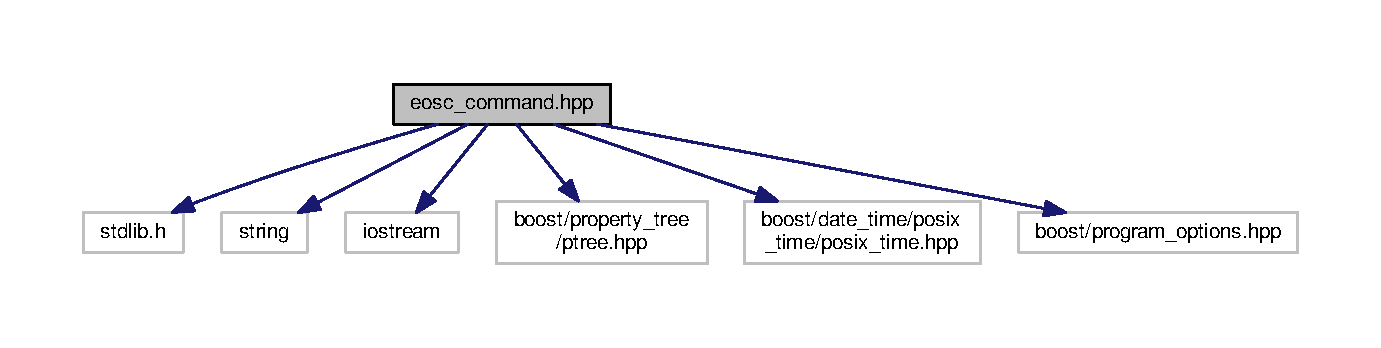
\includegraphics[width=350pt]{eosc__command_8hpp__incl}
\end{center}
\end{figure}
This graph shows which files directly or indirectly include this file\+:
\nopagebreak
\begin{figure}[H]
\begin{center}
\leavevmode
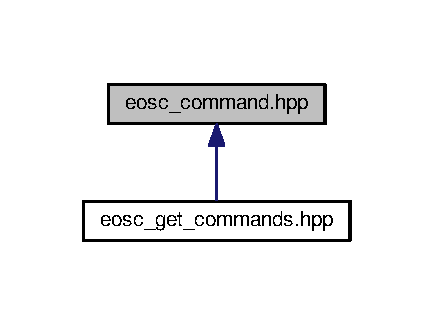
\includegraphics[width=208pt]{eosc__command_8hpp__dep__incl}
\end{center}
\end{figure}
\subsection*{Data Structures}
\begin{DoxyCompactItemize}
\item 
class \hyperlink{classtokenika_1_1eosc_1_1_eosc_command}{tokenika\+::eosc\+::\+Eosc\+Command}
\begin{DoxyCompactList}\small\item\em Basic connection to the blockchain. \end{DoxyCompactList}\item 
class \hyperlink{classtokenika_1_1eosc_1_1_command_options}{tokenika\+::eosc\+::\+Command\+Options}
\begin{DoxyCompactList}\small\item\em Command-\/line wrapper for eosc commands. \end{DoxyCompactList}\end{DoxyCompactItemize}
\subsection*{Macros}
\begin{DoxyCompactItemize}
\item 
\mbox{\Hypertarget{eosc__command_8hpp_a8fe83ac76edc595f6b98cd4a4127aed5}\label{eosc__command_8hpp_a8fe83ac76edc595f6b98cd4a4127aed5}} 
\#define {\bfseries E\+R\+R\+OR}~\char`\"{}error\char`\"{}
\end{DoxyCompactItemize}
\subsection*{Functions}
\begin{DoxyCompactItemize}
\item 
boost\+::posix\+\_\+time\+::ptime {\bfseries tokenika\+::eosc\+::str\+To\+Time} (const std\+::string str)
\begin{DoxyCompactList}\small\item\em Converts E\+OS time string to \textquotesingle{}boost\+::posix\+\_\+time\textquotesingle{}. \end{DoxyCompactList}\item 
void {\bfseries tokenika\+::eosc\+::output} (const char $\ast$label, const char $\ast$format,...)
\begin{DoxyCompactList}\small\item\em Printout formater. \end{DoxyCompactList}\item 
bool {\bfseries tokenika\+::eosc\+::eosc\+Command\+Json} (std\+::string path, boost\+::property\+\_\+tree\+::ptree \&post\+Json, boost\+::property\+\_\+tree\+::ptree \&json\+Rcv)
\begin{DoxyCompactList}\small\item\em Given a json, gets E\+OS blockchain responce. \end{DoxyCompactList}\item 
void {\bfseries tokenika\+::eosc\+::call\+Eosd} (std\+::string server, std\+::string port, std\+::string path, boost\+::property\+\_\+tree\+::ptree \&post\+Json, boost\+::property\+\_\+tree\+::ptree \&json\+Rcv)
\begin{DoxyCompactList}\small\item\em Given a json, gets E\+OS blockchain responce. \end{DoxyCompactList}\item 
{\footnotesize template$<$typename Type $>$ }\\Type {\bfseries tokenika\+::eosc\+::get\+Json\+Path} (boost\+::property\+\_\+tree\+::ptree json, const boost\+::property\+\_\+tree\+::ptree\+::path\+\_\+type \&path)
\begin{DoxyCompactList}\small\item\em Given a json tree, returns the $<$\+Type$>$value of a given path. \end{DoxyCompactList}\item 
boost\+::property\+\_\+tree\+::ptree {\bfseries tokenika\+::eosc\+::string\+To\+Ptree} (std\+::string json)
\begin{DoxyCompactList}\small\item\em Given a text json tree, returns the equivalent {\ttfamily boost ptree}. \end{DoxyCompactList}\end{DoxyCompactItemize}


\subsection{Detailed Description}
Tool for sending transactions and querying state from E\+OS blockchain. 

\begin{DoxyCopyright}{Copyright}
defined in resources/\+L\+I\+C\+E\+N\+S\+E.\+txt Base definitions.
\end{DoxyCopyright}
Defines base classes of the project, and helper methods. 

\subsection{Function Documentation}
\mbox{\Hypertarget{eosc__command_8cpp_file_a522ae193d4a10cba97e59df169dd1da5}\label{eosc__command_8cpp_file_a522ae193d4a10cba97e59df169dd1da5}} 
\index{eosc\+\_\+command.\+hpp@{eosc\+\_\+command.\+hpp}!call\+Eosd@{call\+Eosd}}
\index{call\+Eosd@{call\+Eosd}!eosc\+\_\+command.\+hpp@{eosc\+\_\+command.\+hpp}}
\subsubsection{\texorpdfstring{call\+Eosd()}{callEosd()}}
{\footnotesize\ttfamily void tokenika\+::eosc\+::call\+Eosd (\begin{DoxyParamCaption}\item[{std\+::string}]{server,  }\item[{std\+::string}]{port,  }\item[{std\+::string}]{path,  }\item[{boost\+::property\+\_\+tree\+::ptree \&}]{post\+Json,  }\item[{boost\+::property\+\_\+tree\+::ptree \&}]{json\+Rcv }\end{DoxyParamCaption})}



Given a json, gets E\+OS blockchain responce. 

Given a json tree and a command path (for example {\ttfamily /v1/chain/\+Get\+Info}), and E\+OS blockchain communication port (for example {\ttfamily 8888}), and E\+OS blockchain server name (for example {\ttfamily localhost}), gets E\+OS blockchain responce.


\begin{DoxyParams}{Parameters}
{\em server} & E\+OS blockchain server name \\
\hline
{\em port} & E\+OS blockchain communication port \\
\hline
{\em path} & command path \\
\hline
{\em post\+Json} & json to be posted \\
\hline
{\em json\+Rcv} & json to be filled with received data \\
\hline
\end{DoxyParams}
\mbox{\Hypertarget{eosc__command_8cpp_file_a1c991d7e20076d61c60f1157357eaa9b}\label{eosc__command_8cpp_file_a1c991d7e20076d61c60f1157357eaa9b}} 
\index{eosc\+\_\+command.\+hpp@{eosc\+\_\+command.\+hpp}!eosc\+Command\+Json@{eosc\+Command\+Json}}
\index{eosc\+Command\+Json@{eosc\+Command\+Json}!eosc\+\_\+command.\+hpp@{eosc\+\_\+command.\+hpp}}
\subsubsection{\texorpdfstring{eosc\+Command\+Json()}{eoscCommandJson()}}
{\footnotesize\ttfamily bool tokenika\+::eosc\+::eosc\+Command\+Json (\begin{DoxyParamCaption}\item[{std\+::string}]{path,  }\item[{boost\+::property\+\_\+tree\+::ptree \&}]{post\+Json,  }\item[{boost\+::property\+\_\+tree\+::ptree \&}]{json\+Rcv }\end{DoxyParamCaption})}



Given a json, gets E\+OS blockchain responce. 

Given a json and a command path, for example {\ttfamily /v1/chain/\+Get\+Info}, gets E\+OS blockchain responce.


\begin{DoxyParams}{Parameters}
{\em path} & command path \\
\hline
{\em post\+Json} & json posted \\
\hline
{\em json\+Rcv} & json received \\
\hline
\end{DoxyParams}
\begin{DoxyReturn}{Returns}
true if E\+OS blockchain responce is normal 

false if E\+OS blockchain responce is not normal 
\end{DoxyReturn}
\mbox{\Hypertarget{eosc__command_8cpp_file_a2d300c178b2b0dd2e1762fc6c14ee6e1}\label{eosc__command_8cpp_file_a2d300c178b2b0dd2e1762fc6c14ee6e1}} 
\index{eosc\+\_\+command.\+hpp@{eosc\+\_\+command.\+hpp}!get\+Json\+Path@{get\+Json\+Path}}
\index{get\+Json\+Path@{get\+Json\+Path}!eosc\+\_\+command.\+hpp@{eosc\+\_\+command.\+hpp}}
\subsubsection{\texorpdfstring{get\+Json\+Path()}{getJsonPath()}}
{\footnotesize\ttfamily template$<$typename Type $>$ \\
Type tokenika\+::eosc\+::get\+Json\+Path (\begin{DoxyParamCaption}\item[{boost\+::property\+\_\+tree\+::ptree}]{json,  }\item[{const boost\+::property\+\_\+tree\+::ptree\+::path\+\_\+type \&}]{path }\end{DoxyParamCaption})}



Given a json tree, returns the $<$\+Type$>$value of a given path. 


\begin{DoxyTemplParams}{Template Parameters}
{\em Type} & type of the called value \\
\hline
\end{DoxyTemplParams}

\begin{DoxyParams}{Parameters}
{\em json} & json tree \\
\hline
{\em path} & path of the given tree \\
\hline
\end{DoxyParams}
\begin{DoxyReturn}{Returns}
Type 
\end{DoxyReturn}
\mbox{\Hypertarget{eosc__command_8cpp_file_a03be7086d7980dc8c27b7aaaf8973771}\label{eosc__command_8cpp_file_a03be7086d7980dc8c27b7aaaf8973771}} 
\index{eosc\+\_\+command.\+hpp@{eosc\+\_\+command.\+hpp}!output@{output}}
\index{output@{output}!eosc\+\_\+command.\+hpp@{eosc\+\_\+command.\+hpp}}
\subsubsection{\texorpdfstring{output()}{output()}}
{\footnotesize\ttfamily void tokenika\+::eosc\+::output (\begin{DoxyParamCaption}\item[{const char $\ast$}]{label,  }\item[{const char $\ast$}]{format,  }\item[{}]{... }\end{DoxyParamCaption})}



Printout formater. 

For example, {\ttfamily output(\char`\"{}timestamp\char`\"{}, \char`\"{}\%s\char`\"{}, \char`\"{}2017-\/07-\/18\+T20\+:16\+:36\char`\"{})} produces {\ttfamily \#\# timestamp\+: 2017-\/07-\/18\+T20\+:16\+:36}


\begin{DoxyParams}{Parameters}
{\em label} & \\
\hline
{\em format} & \\
\hline
{\em ...} & \\
\hline
\end{DoxyParams}
\mbox{\Hypertarget{eosc__command_8cpp_file_a0ce29794654e913a1069e28530f4fe46}\label{eosc__command_8cpp_file_a0ce29794654e913a1069e28530f4fe46}} 
\index{eosc\+\_\+command.\+hpp@{eosc\+\_\+command.\+hpp}!string\+To\+Ptree@{string\+To\+Ptree}}
\index{string\+To\+Ptree@{string\+To\+Ptree}!eosc\+\_\+command.\+hpp@{eosc\+\_\+command.\+hpp}}
\subsubsection{\texorpdfstring{string\+To\+Ptree()}{stringToPtree()}}
{\footnotesize\ttfamily boost\+::property\+\_\+tree\+::ptree tokenika\+::eosc\+::string\+To\+Ptree (\begin{DoxyParamCaption}\item[{std\+::string}]{json }\end{DoxyParamCaption})}



Given a text json tree, returns the equivalent {\ttfamily boost ptree}. 


\begin{DoxyParams}{Parameters}
{\em json} & \\
\hline
\end{DoxyParams}
\begin{DoxyReturn}{Returns}
boost\+::property\+\_\+tree\+::ptree 
\end{DoxyReturn}
\mbox{\Hypertarget{eosc__command_8cpp_file_af36b60963055656769794bd43927654c}\label{eosc__command_8cpp_file_af36b60963055656769794bd43927654c}} 
\index{eosc\+\_\+command.\+hpp@{eosc\+\_\+command.\+hpp}!str\+To\+Time@{str\+To\+Time}}
\index{str\+To\+Time@{str\+To\+Time}!eosc\+\_\+command.\+hpp@{eosc\+\_\+command.\+hpp}}
\subsubsection{\texorpdfstring{str\+To\+Time()}{strToTime()}}
{\footnotesize\ttfamily boost\+::posix\+\_\+time\+::ptime tokenika\+::eosc\+::str\+To\+Time (\begin{DoxyParamCaption}\item[{const std\+::string}]{str }\end{DoxyParamCaption})}



Converts E\+OS time string to \textquotesingle{}boost\+::posix\+\_\+time\textquotesingle{}. 

E\+OS time is a string, for example {\ttfamily 2017-\/07-\/18\+T20\+:16\+:36}. For processing, it is converted to the boost {\ttfamily ptime}.


\begin{DoxyParams}{Parameters}
{\em str} & E\+OS time string. \\
\hline
\end{DoxyParams}
\begin{DoxyReturn}{Returns}
boost\+::posix\+\_\+time\+::ptime 
\end{DoxyReturn}

%--- End generated contents ---

% Index
\backmatter
\newpage
\phantomsection
\clearemptydoublepage
\addcontentsline{toc}{chapter}{Index}
\printindex

\end{document}
